Una tira elástica idealizada ocupa \(0\le x\le\ell\), con \(\ell=2\) m. Su desplazamiento transversal \(y(x)\), en metros, es positivo en la dirección de una carga uniforme \(q=6\,\mathrm{N/m}\). Para este modelo estático se suministran todas las relaciones necesarias:
\[
M=D y'',\qquad V=M',\qquad V'=q,
\qquad D=1200\,\mathrm{N\,m^2}.
\]
Las primas indican derivadas respecto de \(x\); \(M\) es un momento, \(V\) una fuerza transversal y estas igualdades fijan sus signos.

En \(x=0\), la tira está fijada de modo que no puede desplazarse ni girar: el giro se representa aquí mediante la pendiente \(y'\). El extremo \(x=\ell\) está libre, sin momento ni fuerza transversal aplicada en el propio extremo. Los valores son sintéticos y no se pide comprobar un diseño estructural.

Traduzca estas leyes y apoyos a una EDO para \(y\) con sus condiciones de contorno. Obtenga la deformación, determine el desplazamiento del extremo libre y verifique las leyes y los apoyos. Justifique además por qué esas condiciones determinan una única solución dentro del modelo suministrado.

\Needspace{6.94cm}
\begin{center}
\begin{minipage}{\linewidth}
\centering
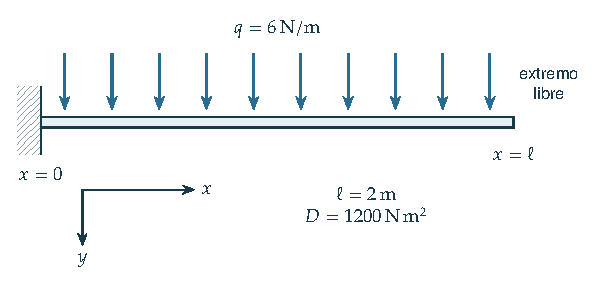
\includegraphics[width=11.34cm]{assets/M2-E0331-setup.pdf}\par
\smallskip{\small Tira empotrada y sentido positivo del desplazamiento transversal.\par}
\end{minipage}
\end{center}
